\documentclass[10pt,a4paper]{article}
\usepackage[english]{babel}
\usepackage[utf8]{inputenc}
\usepackage{amsmath}
\usepackage{amsfonts}
\usepackage{amssymb}
\usepackage{graphicx}
\usepackage{float}
\usepackage{url}
\usepackage{caption}

%link to documentation: 
%https://ackrep-doc.readthedocs.io/en/latest/devdoc/contributing_data.html

\begin{document}
	\part*{Model Documentation of the \\ Acrobot} % MUST - Add Model Name 
	
	%%%%%%%%%%%%%%%%%%%%%% NOMENCLATURE %%%%%%%%%%%%%%%%%%%%%%%%%%%
	
	\section{Nomenclature} % MUST
	\subsection{Nomenclature for Model Equations} % MUST
	
	%variables for model equations
	\begin{tabular}{ll}
		$s_i$ & center of gravity distance of the bar for i = 1, 2 \\
		$m_i$ & mass of the bar for i = 1, 2 \\
		$J_i$ & moment of inertia of the bar for i = 1, 2 \\
		$l_1$ & length of the first bar \\
		$g$ & acceleration due to gravity \\
		$p_1$ & angle between the vertically downwards rest position and the first bar \\
		$q_1$ & angle between the first and the second bar \\
		$\dot{p_1}$ & angle velocity of the first bar \\
		$\dot{q_1}$ & angle velocity of the second bar \\
		$\tau_1$ & input force at the joint \\
				
	\end{tabular}
	
	\subsection{Graphic of the Structure}	
	\begin{figure}[H]
		\centering
		\captionsetup{justification=centering, margin=1cm}
		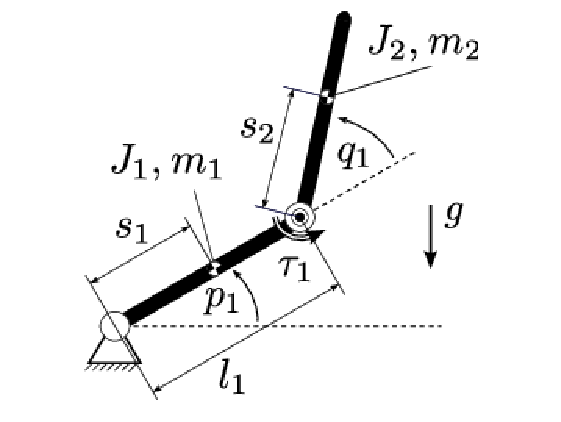
\includegraphics[width=70mm]{acrobot.pdf}
		\caption{Acrobot \\ \footnotesize{Source: Knoll, Carsten/Acrobot (=unteraktuierter Zweigelenkmanipulator, Stellglied im Ellenbogengelenk)}}
	\end{figure}
	 
	%variables which are used additional to those in the model equations
	\begin{tabular}{ll}

	\end{tabular}
	
	%%%%%%%%%%%%%%%%%%%%%% MDOEL EQUATIONS %%%%%%%%%%%%%%%%%%%%%%%%%%%
	
	\section{Model Equations} % MUST
	
	State Vector and Input Vector:
	\begin{align*}
		\underline{x} &= (p_1 \ q_1 \ \dot{p_1} \ \dot{q_1})^T &= (x_1 \ x_2 \ x_3 \ x_4)^T \\
		\underline{u} &= \tau_1 &= u_1
	\end{align*}
	
	\noindent Kinetic Energy:			
	\begin{subequations}
	\begin{align*}
		T &= \frac{J_1x_3^2}{2} + \frac{J_2(x_3 + x_4)^2}{2} + \frac{m_1x_3^2s_1^2 \sin(x_1)^2}{2} + \frac{m_1x_3^2s_1^2 \cos(x_1)^2}{2} \\
		&+ m_2(-l_1x_3 \sin(x_1) - \frac{s_2(x_3 + x_4) \sin(x_1 + x_2))^2}{2} + m_2(l_1x_3 \cos(x_1) \\
		&+ \frac{s_2(x_3 + x_4) \cos(x_1 + x_2))^2}{2}
	\end{align*}
	\end{subequations}
	
	\noindent Potential Energy:			
	\begin{subequations}
	\begin{align*}
		V &= gm_1s_1\sin(x_1) + gm_2(l_1\sin(x_1) + s_2\sin(x_1 + x_2))
	\end{align*}
	\end{subequations}

	%%%%%%%%%%%%%%%%%%%%%% PARAMETERS | OUTPUTS %%%%%%%%%%%%%%%%%%%%%%%%%%%
	\noindent
	Parameters: $s_1, \, s_2, \, m_1, \, m_2, \, J_1 , \, J_2, \, l_1, \, g$ % variables with constant, predefined value
	\\
	Outputs: $\underline{x}$ % MAY
	
	%%%%%%%%%%%%%%%%%%%%%% ASSUMPTIONS %%%%%%%%%%%%%%%%%%%%%%%%%%%
	
	\subsection{Assumptions} % MAY 
		\begin{enumerate} %possible list type for the Assumptions
			\item The rest position of the acrobot is vertically downward.  
		\end{enumerate}
	
	%%%%%%%%%%%%%%%%%%%%%% EXEMPLARY PARAMETER VALUES %%%%%%%%%%%%%%%%%%%%%%%%%%%	
	
	\subsection{Exemplary parameter values}
	\begin{tabular}{cl}
\hline
  Symbol  & Value                                                                                                                                                                                \\
\hline
   $A$    & $\left[\begin{matrix}0.8189 & 0.0863 & 0.09 & 0.0813\\0.2524 & 1.0033 & 0.0313 & 0.2004\\-0.0545 & 0.0102 & 0.7901 & -0.258\\-0.1918 & -0.1034 & 0.1602 & 0.8604\end{matrix}\right]$ \\
   $B$    & $\left[\begin{matrix}0.0045 & 0.0044\\0.1001 & 0.01\\0.0003 & -0.0136\\-0.0051 & 0.0936\end{matrix}\right]$                                                                          \\
 $B_{1}$  & $\left[\begin{matrix}0.0045 & 0.0044\\0.1001 & 0.01\\0.0003 & -0.0136\\-0.0051 & 0.0936\end{matrix}\right]$                                                                          \\
 $C_{1}$  & $\left[\begin{matrix}1.0 & 0 & -1.0 & 0\\0 & 0 & 0 & 0\\0 & 0 & 0 & 0\end{matrix}\right]$                                                                                            \\
   $C$    & $\left[\begin{matrix}1.0 & 0 & 0 & 0\\0 & 0 & 1.0 & 0\end{matrix}\right]$                                                                                                            \\
 $D_{11}$ & $\left[\begin{matrix}0 & 0 & 0\\0 & 0 & 0\\0 & 0 & 0\end{matrix}\right]$                                                                                                             \\
 $D_{12}$ & $\left[\begin{matrix}0 & 0\\1.0 & 0\\0 & 1.0\end{matrix}\right]$                                                                                                                     \\
 $D_{21}$ & $\left[\begin{matrix}0 & 1.0 & 0\\0 & 0 & 1.0\end{matrix}\right]$                                                                                                                    \\
\hline
\end{tabular}

	%%%%%%%%%%%%%%%%%%%%%% DERIVATION & EXPLANATION %%%%%%%%%%%%%%%%%%%%%%%%%%%	
	
	\section{Derivation and Explanation} % SHOULD
	The Lagrangian mechanics was used for the solution.
	
	
	%%%%%%%%%%%%%%%%%%%%%% REFERENCES %%%%%%%%%%%%%%%%%%%%%%%%%%%
	
	\begin{thebibliography}{10}		
		\bibitem{But21}Knoll, Carsten: 
		\textit{Acrobot (=unteraktuierter Zweigelenkmanipulator, Stellglied im Ellenbogengelenk)}, Jupyter Notebook published 2017. \\
		\url{https://github.com/cknoll/beispiele/blob/master/acrobot_rwa.ipynb}
	\end{thebibliography}

\end{document}

